\graphicspath{ {./content/results/figures/} }

\section{Results}
\label{sec:res}

\subsection{Qualitative}

\begin{figure}
  \centering
  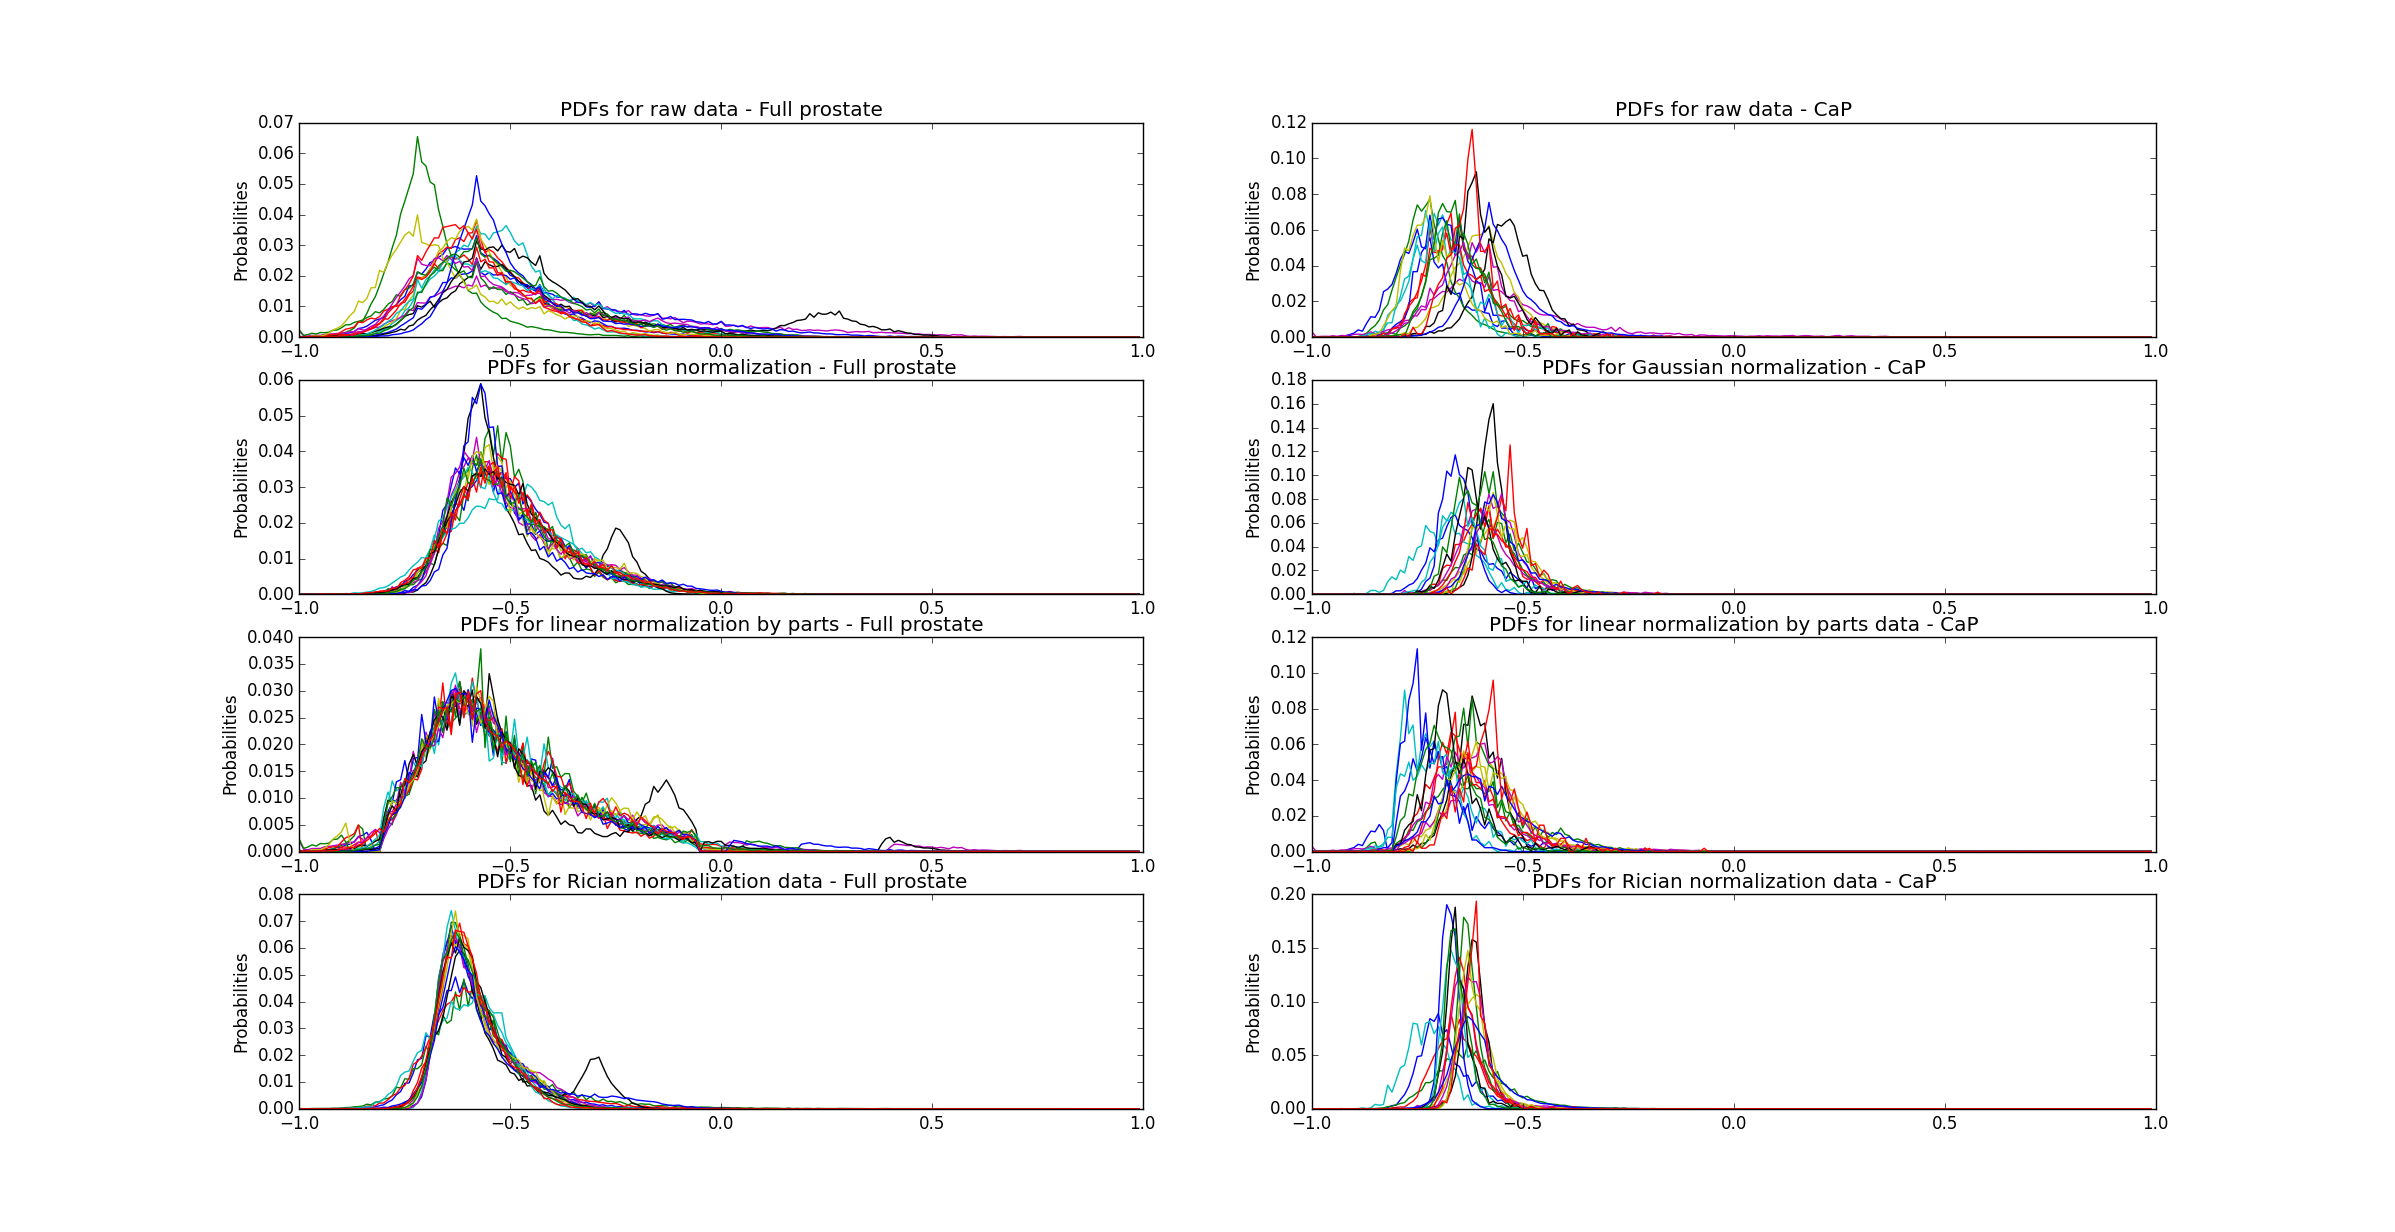
\includegraphics[width=1.\textwidth]{qualitative.png}
  \caption{Qualitative evaluation by visual inspection of the alignment of the \ac{pdf}s for the full prostate and the \ac{cap}.}
  \label{fig:qu}
\end{figure}

Figure~\ref{fig:qu} depicts the alignment of the different \ac{pdf}s using the different methods implemented. 
All the methods seem to address the problem of the \ac{pdf} alignment of the full prostate data.
However, the Rician normalization seems to outperform the other methods when focusing solely on the \ac{cap} data.
The \ac{pdf} computed in this specific area is more skewed from its original shape in the case of the piecewise-linear normalization than with the three other normalization strategies.
The \ac{srsf} normalization gets unstable due to the warping function $\gamma$ found which is in practise non-smooth.

\subsection{Quantitative}

\begin{figure*}
  \centering
  \subfloat[][]{
    \label{fig:qtfull}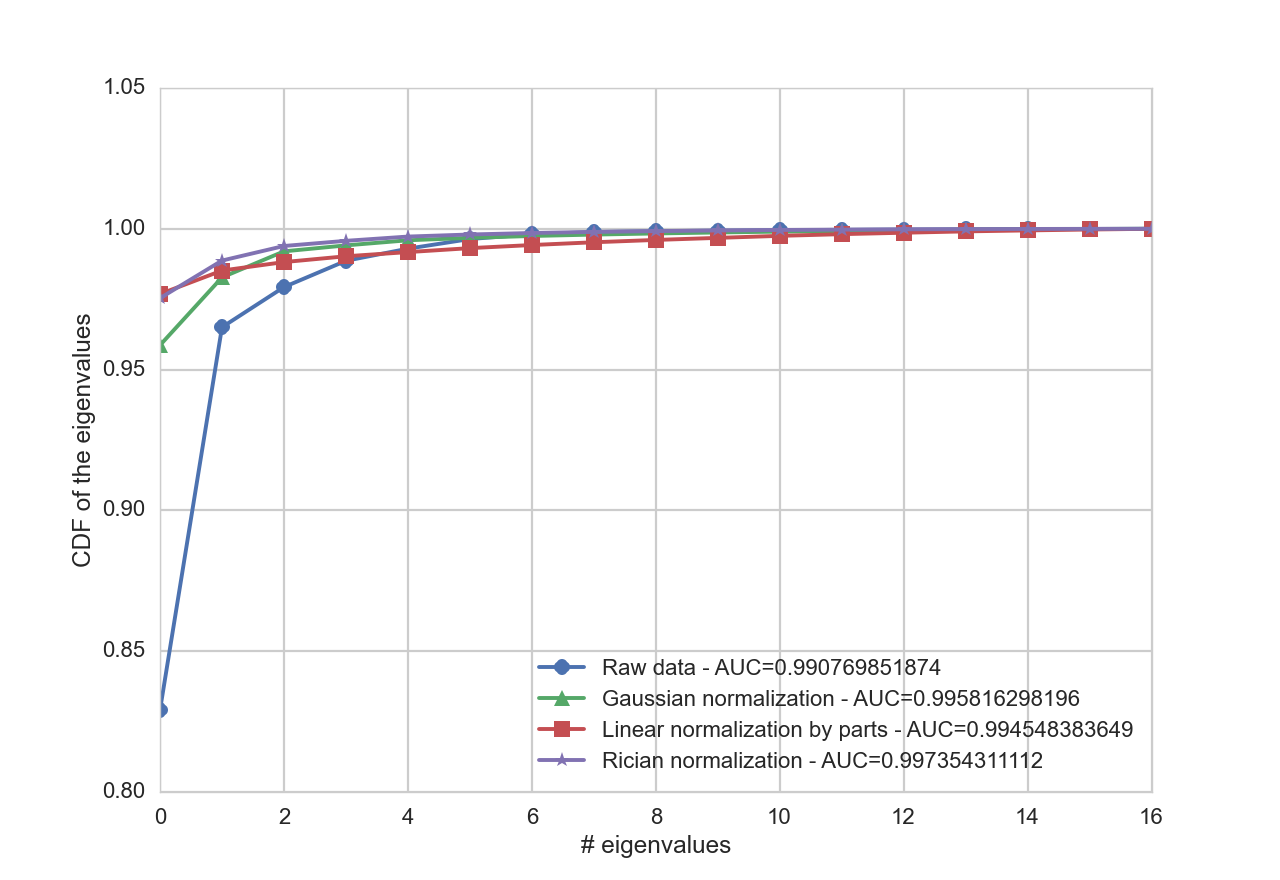
\includegraphics[width=0.48\textwidth]{quantitative_1.png}}\hfill
  \subfloat[][]{
    \label{fig:qtcap}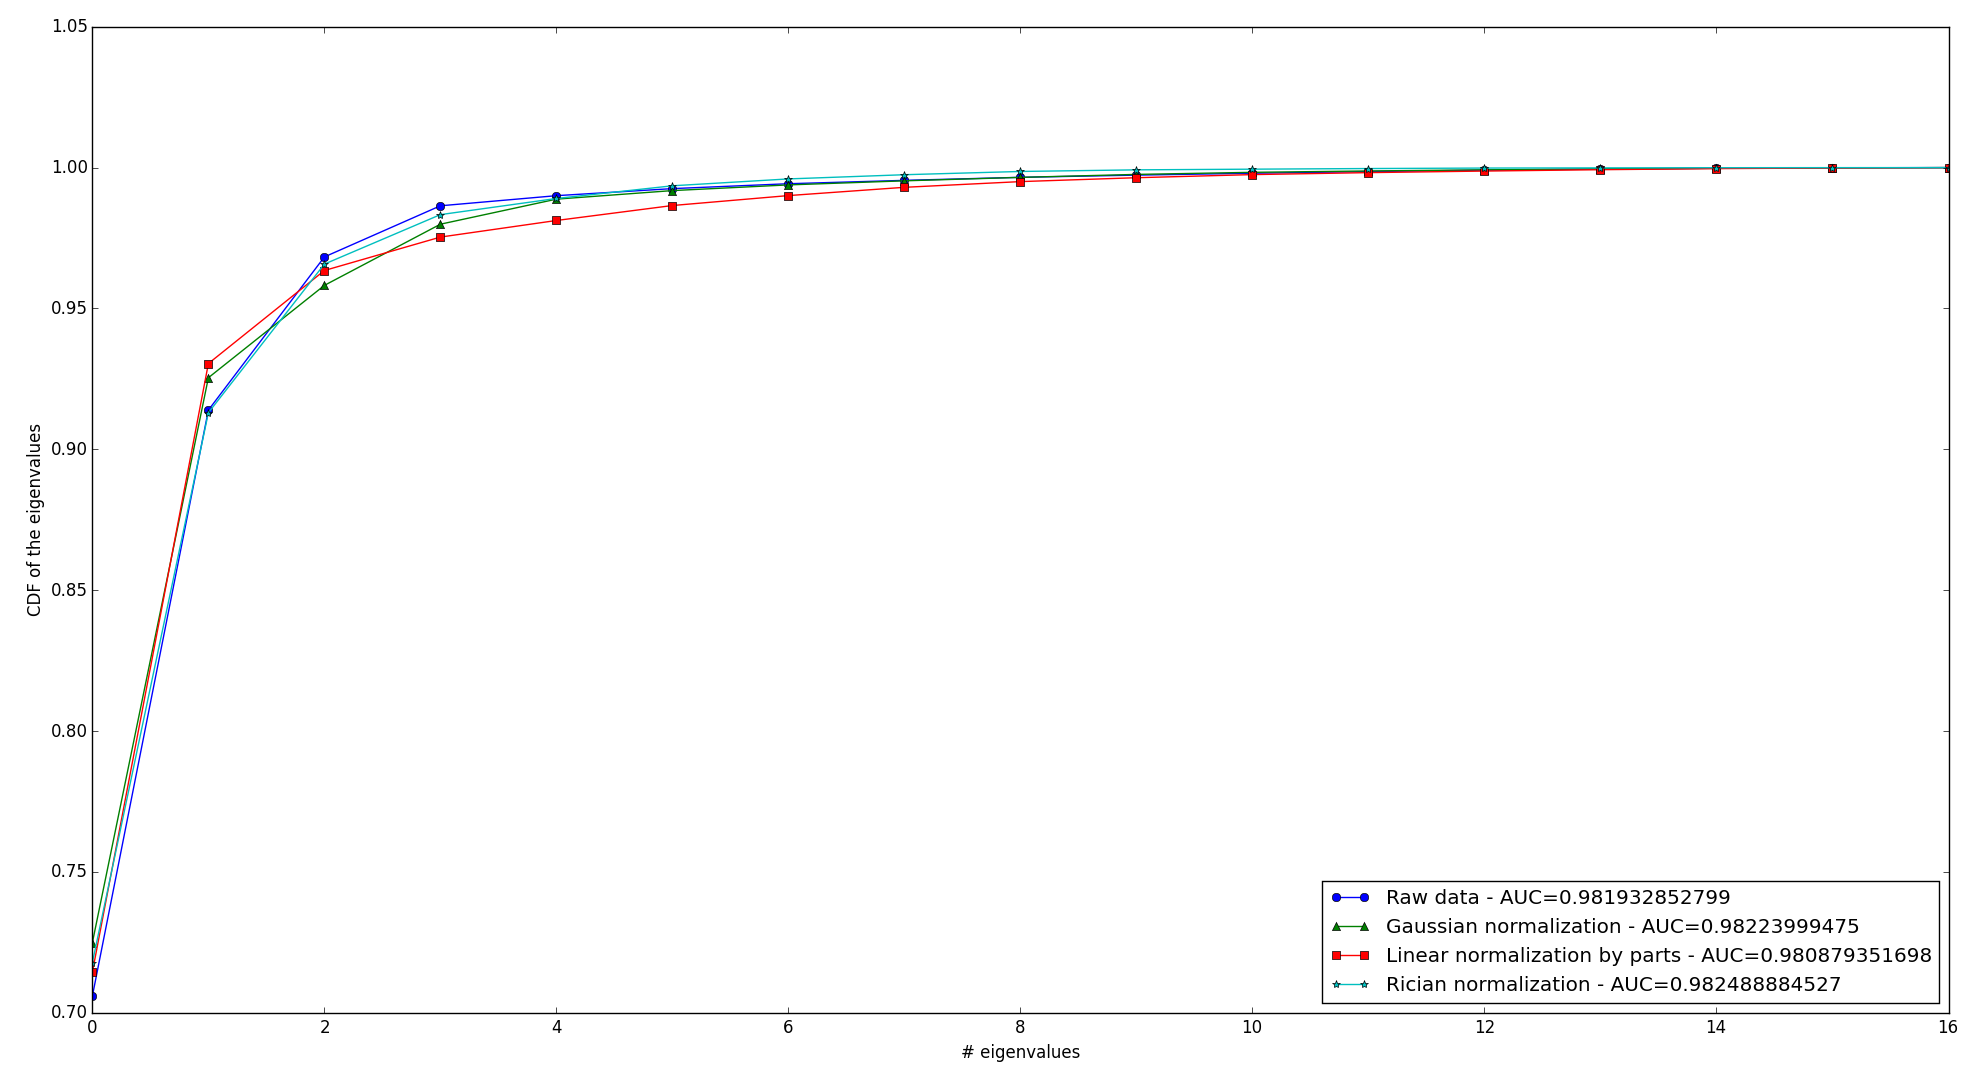
\includegraphics[width=0.48\textwidth]{quantitative_2.png}}
  \caption{Spectral evaluation using \ac{pca} decomposition: \protect\subref{fig:qtfull} evaluation considering the full prostate, \protect\subref{fig:qtcap} evaluation considering only the \ac{cap}.}
  \label{fig:qt}
\end{figure*}

A spectral evaluation is performed by decomposing the set of normalized \ac{pdf}s using \ac{pca} under the assumption that they are linearly dependent. 
Intuitively, the eigenvalues of the \ac{pca} decomposition are correlated with the alignment of the different \ac{pdf}s.
Thus, in the case of a perfect alignment of the \ac{pdf}s, the first eigenvalue is much greater than the remaining since that the first eigenvector encodes all the information.
In the contrary, in the case of a misalignment of the \ac{pdf}s, more eigenvectors are needed to encode the information synonymous with larger eigenvalues.
Thus, we propose to use the cumulative sum of the normalized eigenvalues as well as the \ac{auc}, as depicted in Fig.\,\ref{fig:qt}.
Rician normalization outperforms the other methods with an \ac{auc} of $0.9974$ and $0.9824$ considering the full prostate and \ac{cap}, respectively.

%%% Local Variables: 
%%% mode: latex
%%% TeX-master: "../../master"
%%% End: 
